\section{The RoXOR Protocol}
\label{sec:htproblem}
In this section, we provide details of how RoXOR encodes the incremental redundancy and how RoXOR jointly decodes the retransmitted packet and the original corrupted packet using successive interference cancellation.Throughout our discussion, we assume that the network operates at a high SNR so that most packet errors are due to interference from other users. We assume no side information and focus on a protocol based on retransmissions.

\subsection{Structured Encoding}
One of the code parameters is $\beta$, $0\leq\beta\leq1$, which controls the amount of incremental redundancy. For a length $L$ packet, the original information bits are given by samples $x_1,x_2,...,x_L$ while the code bits are given by $c_1,c_2,...,c_n$. For a parameter $\beta$, the length of the codeword becomes $int(\beta n)$. Therefore, the final code is given by:
\begin{equation}
c_i = 
\begin{cases}
x_{i} + x_{L-i} & \beta \leq 0.5 \\
x_{i} + x_{i+\frac{L}{2}} & \beta > 0.5
\end{cases}
\end{equation}

	
\emph{How is Folding Applied for (Degree n)?} 
\begin{itemize}
    \item Maximum Distance between any 2 data symbols is defined as: $D_{m}\doteq int(\frac{N}{n})$.
    \item Step size s, $s\doteq mod(i-1,D_m)$.
    \item Increment size t, $t\doteq mod(int(\frac{i}{D_m}),n)$
\end{itemize}

\begin{equation}
        c_i = \begin{cases}
                \sum_{k=0}^{n-1}x_{1+s+(D_m-t)k} & s \leq \frac{D_m}{2} \\
                \sum_{k=0}^{n-1}x_{N-s+(D_m-t)k} & s > \frac{D_m}{2}
        \end{cases}
\end{equation}

%Generalizing, define $\beta=\frac{L}{N}$, as the degree of the incremental redundancy. For example a degree-two code uses the binary addition of two data bits in the original packet for one code-bit of the retransmitted packet. 

\subsection{Structured Decoding}
\label{sec:DecodeSection}

\begin{figure}[t]
	\label{fig:roxor_decode}	
	\centering
	\vspace*{-0.1in}
	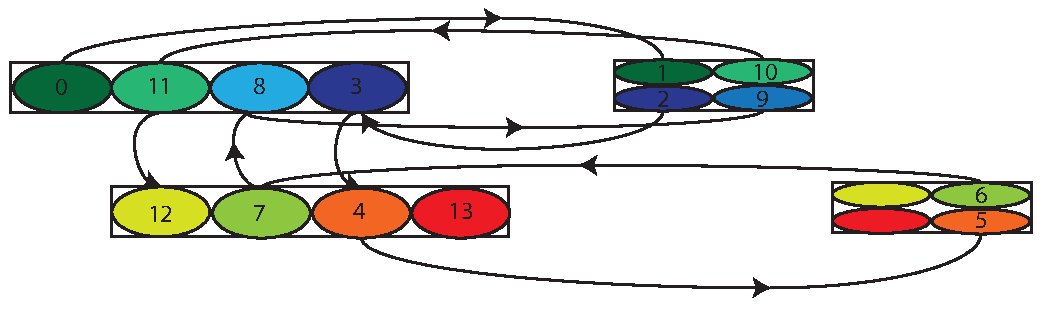
\includegraphics[width=.9\columnwidth]{./figs/roxor_timing_diagram_decoding.pdf}
	\vskip -0.5em
	\caption{The RoXOR decoding process for $\beta=0.5$}
	\vskip -1em
\end{figure}

The decoding process is illustrated in figure~\ref{fig:roxor_decode} where the numbers on the bubbles indicate the particular decode order. This figure shows the original packet being interfered with and the smaller re-transmitted packets of size $\beta$. First, the clean portions of both the transmitted packets are decoded, and then the system applies successive interference cancellation to iteratively decode previously corrupted chunks. This process continues until all of the bits from the original packets are decoded and pass the CRC check. This example, although simplified, gives intuition behind the RoXOR decoding process. Furthermore, it shows that it is rather conservative to send 100\% of the original packet on re-transmission, as RoXOR was able to decode using only about 50\%.

\subsection{Small Packet Sizes}
\label{sec:small_packet}

\begin{enumerate}
    \item In the case of small packets, the re-transmission overhead could be significant.
    \item When the MAC overhead is not negligible is it better to send using a stronger FEC?
    \item The most appropriate type of FEC would be a burst error correction code. 
\end{enumerate}

\textbf{Rieger Bound} Consider a linear code with parameters $(n,k)$, where $k$ is the information block size, and $n$ is the code block size. The burst error correcting ability of an $(n,k)$ linear block code is then $2l \leq n-k$, therefore:
\begin{equation}
l \leq \frac{(n-k)}{2}
\end{equation}

\begin{enumerate}
    \item Assuming we use an optimal burst correction code, which scheme has better mean delay? RoXOR or 802.11x with stronger FEC?
\end{enumerate}

\subsection{Large Packet Sizes}
\label{sec:large_packet}

\begin{enumerate}
    \item For large packet sizes, MAC overhead is negligible, hence, it is reasonable to send a re-transmission packet more than once.
\end{enumerate}

\subsection{Three or More Users}
\label{sec:three_users}

\begin{enumerate}
	\item How does this work with 3 or more users?
	\begin{enumerate}
		\item Folding using degree 2 performs similarly to random codes of degree $4\sim6$.
	\end{enumerate}

 \end{enumerate}

